\documentclass[11pt]{article}

\usepackage{thumbpdf, amssymb, amsmath, amsthm, microtype,
	    graphicx, verbatim, listings, color, fancybox}
\usepackage[pdftex]{hyperref}
%\usepackage[margin=1in]{geometry}
\usepackage{cawsty}
\usepackage{fullpage}
\usepackage{pseudocode}
\usepackage{verbatim}
\usepackage{multicol}

\usepackage{fancybox}
\usepackage{tikz}

\newcommand{\tlg}{\text{lg}}
\newcommand{\tln}{\text{ln}}
\newcommand{\tlog}{\text{log}}

\usepackage{algorithm}
%\usepackage{algorithmic}
\usepackage{amsmath}
\usepackage{amsthm}
\usepackage{algpseudocode}
\usepackage{algorithmicx}% http://ctan.org/pkg/algorithmicx
\usepackage{lipsum}% http://ctan.org/pkg/lipsum
\usepackage{xifthen}% http://ctan.org/pkg/xifthen
\usepackage{needspace}% http://ctan.org/pkg/needspace
\usepackage{hyperref}% http://ctan.org/pkg/hyperref

\usepackage{tikz}
\usetikzlibrary{arrows,%
                shapes,positioning}

\tikzstyle{vertex}=[circle,fill=black!25,minimum size=20pt,inner sep=0pt]
\tikzstyle{selected vertex} = [vertex, fill=red!24]
\tikzstyle{edge} = [draw,thick,-]
\tikzstyle{weight} = [font=\small]
\tikzstyle{selected edge} = [draw,line width=5pt,-,red!50]
\tikzstyle{ignored edge} = [draw,line width=5pt,-,black!20]

\allowdisplaybreaks[1]

% ================ ALGORITHM ENVIRONMENT ================
\newcounter{numberedAlg}% Algorithm counter
\newenvironment{numberedAlg}[1][]%
  {% \begin{numberedAlg}[#1]
    \needspace{2\baselineskip}% At least 2\baselineskip required, otherwise break
    \noindent \rule{\linewidth}{1pt} \endgraf% Top rule
    \refstepcounter{numberedAlg}% For correct reference of algorithm
    \centering \textsc{Algorithm}~\thenumberedAlg%
    \ifthenelse{\isempty{#1}}{}{:\ #1}% Typeset name (if provided)
  }{% \end{numberedAlg}
  \noindent \rule{\linewidth}{1pt}% Bottom rule
  }%

%\setlength{\parindent}{0pt}

\linespread{1.2}

\begin{document}
\cawtitle{4005-800 Algorithms}{Homework 7}

\begin{prob}{1 - 34.2-1}
Consider the language GRAPH-ISOMORPHISM = $\{\langle G_1, G_2 \rangle : G_1$ and $G_2$ are isomorphic graphs $\}$. Prove that GRAPH-ISOMORPHISM $\in NP$ by describing a polynomial-time algorithm to verify the language.
\end{prob}
\begin{sol}
By the defintion of graph isomorphism, two graphs $G_1$ and $G_2$ are isomorphic if and only if there exists a bijection $m : V(G_1) \to V(G_2)$ such that any two vertices $v_i$ and $v_j$ of $G_1$ are adjacent in $G_1$ if and only if $m(v_i)$ and $m(v_j)$ are adjacent in $G_2$. With this definition, it is enough to check the bijection $m$ to see if it fulfills this property to verify that two graphs isomorphic. We can easily devise a polynomial-time algorithm to solve this as follows:

\begin{numberedAlg}[GRAPH-ISOMORPHISM-VERIFIER]
\label{alg1}
\begin{algorithmic}[1]
	\Function{VerifyGraphIsomorphism}{$m$}
		\ForAll{$v_{i} \in V(G_1)$}
			\State vCount = 0 \Comment {Count number of times $v_i$ appears in $G_2$}
			\ForAll{$v_j \in V(G_2)$}
				\If{$m(v_i) == v_j$}
					\State vCount = vCount + 1
				\EndIf
			\EndFor
			\If {vCount $\not= 1$} \Comment {$v_i$ should only appear once in $G_2$}
				\State \Return False
			\EndIf
		\EndFor
\\
		\ForAll{$v_i \in V(G_1)$}
			\ForAll{$v_j \in V(G_1)$}
				\If{$(v_i, v_j) \in E(G_1)$ and $(m(v_i), m(v_j)) \notin E(G_2)$}
					\State \Return False
				\EndIf
			\EndFor
		\EndFor
\\
		\ForAll{$v_i \in V(G_1)$}
			\ForAll{$v_j \in V(G_1)$}
				\If{$(m(v_i), m(v_j)) \in E(G_2)$ and $(v_i, v_j) \notin E(G_1)$}
					\State \Return False
				\EndIf
			\EndFor
		\EndFor
\\
		\State \Return True
	\EndFunction
\end{algorithmic}
\end{numberedAlg}

Note that $m$ denotes the bijective mapping (the permutation) from $V(G_1)$ to $V(G_2)$. It is clear that the permutation check runs in $O(V)$ time and the edge check runs in $O(V^2)$ time. Thus, we conclude that this algorithms runs in $O(V^2)$ time and thus verifies the solution (i.e. the permutation mapping $m$) to the GRAPH-ISOMORPHISM problem in polynomial time. 
\end{sol}

\begin{prob}{2 - 34.2-10}
Prove that if $NP \not= co$-$NP$, then $P \not= NP$.
\end{prob}
\begin{sol}
If $NP \not= co$-$NP$, then we know there exists a problem $Q \in NP$ such that $Q \notin co$-$NP$.  Furthermore, by definition, we know that $P \in co$-$NP \cap NP$. Now, let $Q$ be a problem in $NP$ that is not in $co$-$NP$. By the definition of the set intersection, that means that $Q \notin co$-$NP \cap NP$, and thus we know that $Q \in NP$ and $Q \notin P$ (becuse $P$ is a subset of $co$-$NP \cap NP$). Therefore, since there exists a problem that is in $NP$ but not in $P$, we conclude that $P \not= NP$. 
\end{sol}

\begin{prob}{3 - 34.3-1}
Verify that the circuit in Figure $34.8(b)$ is unsatisfiable.
\end{prob}
\begin{sol}
\begin{center}
	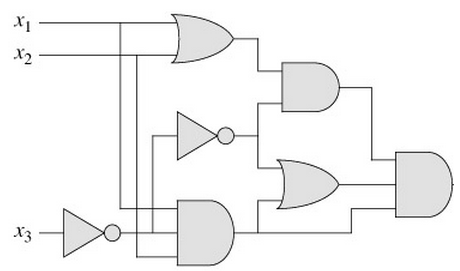
\includegraphics[scale=0.5]{circuit.png} \\
\end{center}

The logical equivalent expression for this circuit is as follows:
\begin{eqnarray*}
((x_1 \lor x_2) \land x_3) \land (x_3 \lor (x_1 \land x_2 \land \lnot x_3)) \land (x_1 \land x_2 \land \lnot x_3)
\end{eqnarray*}

To show that this circuit is unsatisfiable, we simply build a truth table for the boolean expression that considers all logical values for $x_1, x_2,$ and $x_3$, as shown in table \ref{thetable}:

\begin{table}
\centering
    \begin{tabular}{|l|l|l|l|l|l|}
        \hline
        $x_1, x_2, x_3$ & $x_1 \lor x_2$ & $(x_1 \lor x_2) \land x_3$ & $x_1 \land x_2 \land \lnot x_3$ & $x_3 \lor (x_1 \land x_2 \land \lnot x_3)$ & Final AND Gate \\ \hline
        F,F,F & F & F & F & F & F \\ 
        F,F,T & F & F & F & T & F \\ 
        F,T,F & T & F & F & F & F \\ 
        F,T,T & T & T & F & T & F \\ 
        T,F,F & T & F & F & F & F \\ 
        T,F,T & T & T & F & T & F \\ 
        T,T,F & T & F & T & T & F \\ 
        T,T,T & T & T & F & T & F \\ 
        \hline
    \end{tabular}
	\label{thetable}
	\caption{Truth table for problem \#3, where T = True and F = False.}
\end{table}

Therefore, since there is no possible combination of logical values for $x_1$, $x_2$, and $x_3$ such that the boolean expression is true, we conclude that it is unsatisfiable.

\end{sol}

\begin{prob}{4 - 34.4-5}
Show that the problem of determining the satisfiability of boolean formulas in disjunctive normal form is polynomial-time solvable.
\end{prob}
\begin{sol}
We show that the problem of determining the satisfiability of boolean formulas in disjunctive normal form is polynomial-time solvable by providing a polynomial-time algorithm that performs this task. This algorithm is realized below in Algorithm \ref{alg2}.

\begin{numberedAlg}[DNF-SOLVER]
\label{alg2}
\begin{algorithmic}[1]
	\Function{SolveDNF}{$\psi$}
		\ForAll{$v_{i} \in V(G_1)$}
			\State vCount = 0 \Comment {Count number of times $v_i$ appears in $G_2$}
			\ForAll{$v_j \in V(G_2)$}
				\If{$m(v_i) == v_j$}
					\State vCount = vCount + 1
				\EndIf
			\EndFor
			\If {vCount $\not= 1$} \Comment {$v_i$ should only appear once in $G_2$}
				\State \Return False
			\EndIf
		\EndFor
\\
		\State \Return True
	\EndFunction
\end{algorithmic}
\end{numberedAlg}

\end{sol}

\begin{prob}{5 - 34.5-5}
The \textbf{set-partition problem} takes as input a set $S$ of numbers. The question is whether the numbers can be partitioned into two sets $A$ and $A' = S - A$ such that $\sum_{x \in A}x = \sum_{x \in A'} x$. Show that the set-partition problem is $NP$-complete.
\end{prob}
\begin{sol}
In order to show that the set-partition problem, $Q$ is $NP$-complete, we show that it reduces to the subset-sum problem, $Q'$. That is, we prove $Q \leq_p Q'$. 
\end{sol}

\begin{prob}{6}
TODO
\end{prob}
\begin{sol}
\begin{numberedAlg}[RECURSIVE-KNAPSACK]
\label{alg1}
\begin{algorithmic}[1]
	\item TODO
\end{algorithmic}
\end{numberedAlg}
\end{sol}

\end{document}
